Pneumatic mechanism is also a potential solution.
Its main advantage is that the power source is divorced from the actuator \cite{russomanno_design_2015}.
Power, in the form of pressurized air, is routed via small pipes and readily converted into the motion of a sliding pin using an elastic membrane.
This feature of separation of power source and functional module make pneumatic design promising in terms of forming a large-area dense array shape display.
However, one big challenge of pneumatic design is how to efficiently control large number of cells without sacrifice of portability \cite{russomanno_model-based_2017}.
The group proposed a fluidic logic system design shown in figure \ref{fig:pneumatic-schema} and figure \ref{fig:Integrated fluidic logic system} to solve this problem and the application of this model is expected to be able to reduce the required number of external control valves from many thousands (one for each tactile feature) down to just a few \cite{russomanno_design_2015}.

\begin{figure}[ht]\centering
    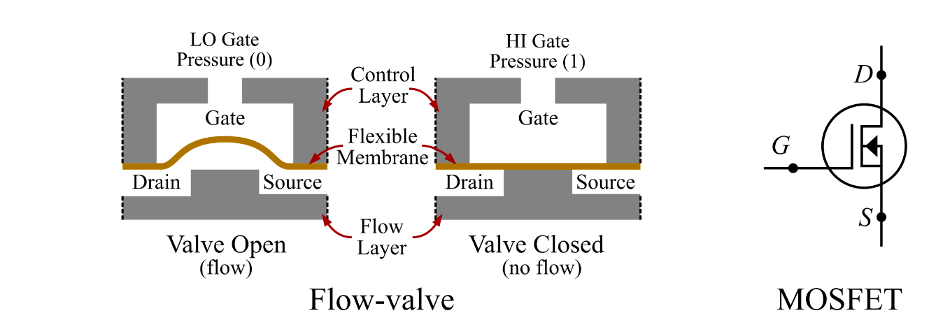
\includegraphics[width=0.6\textwidth]{figures/pneumatic-schema.png}
\caption{Cross-sectional views of a pressure-based fluidic valve in the open and closed states.}
\label{fig:pneumatic-schema}
\end{figure}
\begin{figure}[ht]\centering
    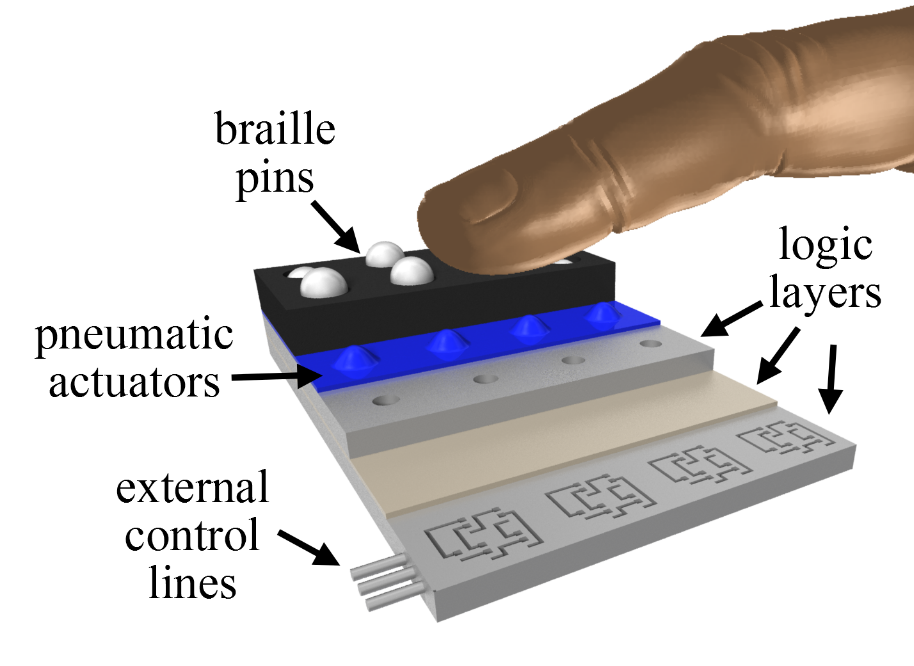
\includegraphics[height=4.5cm]{figures/fluidic logic system.png}
\caption{An integrated fluidic logic and actuator system for surface haptics.}
\label{fig:Integrated fluidic logic system}
\end{figure}

One commercial solution taking advantage of the technology was announced by Blitab, who started pre-orders 2017 but never officially went to market. Their proposed device is shown in figure \ref{fig:Blitab-product}.
In spite of its reasonable end price of USD 500, the complexity of the necessary fluidic logic system combined with the possible complications they must have encountered to have to delay the release of the product, make this design unsuitable for the scope of this project.

\begin{figure}[ht]\centering
    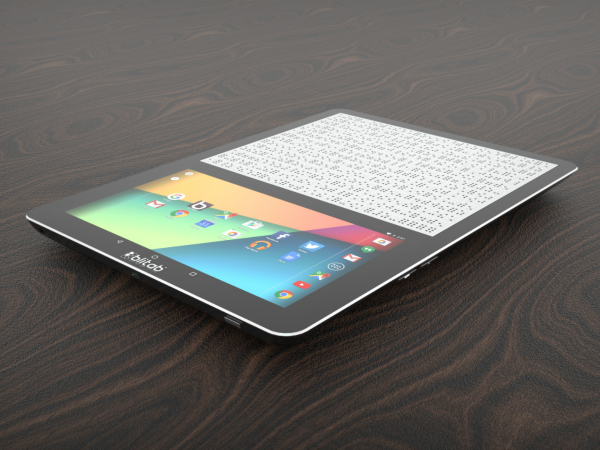
\includegraphics[height=5cm]{figures/Blitab_product.jpg}
\caption[Commercial pneumatic braille display]{Commercially announced though never released pneumatic-based braille display. Combines the capabilities of a smartphone and a 2d dimensional refresible braille display.}
\label{fig:Blitab-product}
\end{figure}